\chapter{Evaluación Experimental}\label{chap:evaluacion}

En los capítulos anteriores se explicaron diferentes métodos de algoritmos de aprendizaje supervisado, redes neuronales y las diversas fuentes de datos para poder entrenar un modelo de detección. En  base a lo desarrollado en las anteriores secciones  explicaremos el proceso de aprendizaje llevado a cabo detallando todos los  experimentos realizados para la construcción del modelo como así también  el proceso de validación y las métricas que se utilizaron para su evaluación. Para finalizar se discutirá todos los resultados obtenidos para cada uno de los  experimentos realizados. 

\section{Datos de entrenamiento}\label{sec:datos_entrenamiento}

Para la construcción del modelo de detección se dividió el datasets en datos de entrenamiento y datos de test para cada datesets de imágenes creado,  para el cual se dividió en 40 imágenes de entrenamiento y 10 imágenes para test. Cada una de las imágenes obtenidas se calculo sus bounding boxes correspondientes  siguiendo el esquema de procesamiento desarrollado  en la sección (Sec:\ref{sec: pipeline}); en promedio se obtuvieron $1500$ bounding boxes por cada una de las imágenes procesadas por lo que el datasets final de entrenamiento fue de $60000$ y el de test de $15000$ regiones en promedio dependiendo de las características de las imágenes procesadas por combinaciones de bandas. 

\subsection{Combinaciones de bandas en canales RGB}\label{sub:comb_de_banda} 
%http://www.gisandbeers.com/combinacion-de-imagenes-satelite-landsat-sentinel-rgb/

%Las redes neuronales que vamos a utilizar para la construcción de esta tesis son redes neuronales pre-entrenadas (Sec:\ref{sub:cnn}), estas redes neuronales necesitan como entrada imágenes ópticas con tres canales correspondiente a \textit{RGB} (rojo, verde y azul), los canales RGB se emplean para representar distintos colores a partir de la mezcla de cada uno de estos.

Las combinaciones de bandas en imágenes satelitales nos ayudan a analizar y diferenciar diferentes elementos dentro de la imagen, para esto utilizamos diversas combinaciones de bandas en base a los canales RGB que nos permiten visualizar diferentes elementos de acuerdo a la banda que estamos utilizando. El paso de cada banda por un canal RGB especifico permitirá teñir de colores los elementos que ofrezcan mayor o menor reflexión de longitudes de onda; como por ejemplo, la vegetación, focos de incendios, agua, brindando diferentes fuentes de información para ser explotada. El conjunto de bandas seleccionadas para los experimentos son las de resolución moderada (M-bands) (\ref{tab:viirs}).
 
Para la construcción del dataset final se utilizaron las bandas impares (\ref{tab:viirs})  mas las bandas que corresponden al color verdadero. En total se obtuvieron 29 datasets con combinaciones de bandas diferentes para realizar la evaluación experimental; en el siguiente cuadro  \ref{tab:combinacion_banda} se puede ver todas las combinaciones de bandas utilizadas para la construcción final del los dataset.

\begin{table}[h] \begin{center}
\begin{tabular}{|c|c||c|c|}\hline 
\textbf{Num} & \textbf{Combinación de banda} & \textbf{Num} & \textbf{Combinación de banda} \\ \hline 
1  	& 	M1-M1-M1 			& 16  & 	M9-M11-M7  \\ \hline
2  	&   M1-M3-M5			& 17  & 	M9-M7-M11\\  \hline
3  	& 	M1-M5-M3			& 18  & 	M11-M11-M11\\ \hline
4  	&   M3-M1-M5 			& 19  & 	M11-M13-M15\\ \hline
5   & 	M3-M3-M3 			& 20  & 	M11-M15-M13\\ \hline
6   & 	M3-M5-M1 			& 21  & 	M13-M11-M15 \\ \hline
7   & 	M5-M1-M3 			& 22  & 	M13-M13-M13\\ \hline
8   & 	M5-M3-M1 			& 23  & 	M13-M15-M11\\ \hline
9   &   M5-M5-M5  			& 24  & 	M15-M11-M13\\ \hline
10  &	M7-M7-M7   			& 25  & 	M15-M13-M11\\ \hline
11  & 	M9-M9-M9   			& 26  & 	M15-M15-M15\\ \hline
12  & 	M11-M7-M9  			& 27  & 	M5-M4-M3\\ \hline
13  & 	M11-M9-M7  			& 28  & 	M10-M7-M5\\ \hline
14  &  	M7-M11-M9  			& 29  & 	M11-M12.M13\\ \hline
15  & 	M7-M9-M11  			& -& -\\ \hline      	
\end{tabular}
\end{center}\caption{Combinaciones de bandas utilizadas \label{tab:combinacion_banda}}
\end{table}

En la siguiente figura \ref{Fig: bandas543} podemos visualizar unas de las imágenes que se utilizo; en este caso corresponde  a las combinaciones de bandas M5, M4, M3 conocidas como color verdadero, \textit{true color} su nombre en ingles .

\begin{figure}[H]
 \centering
  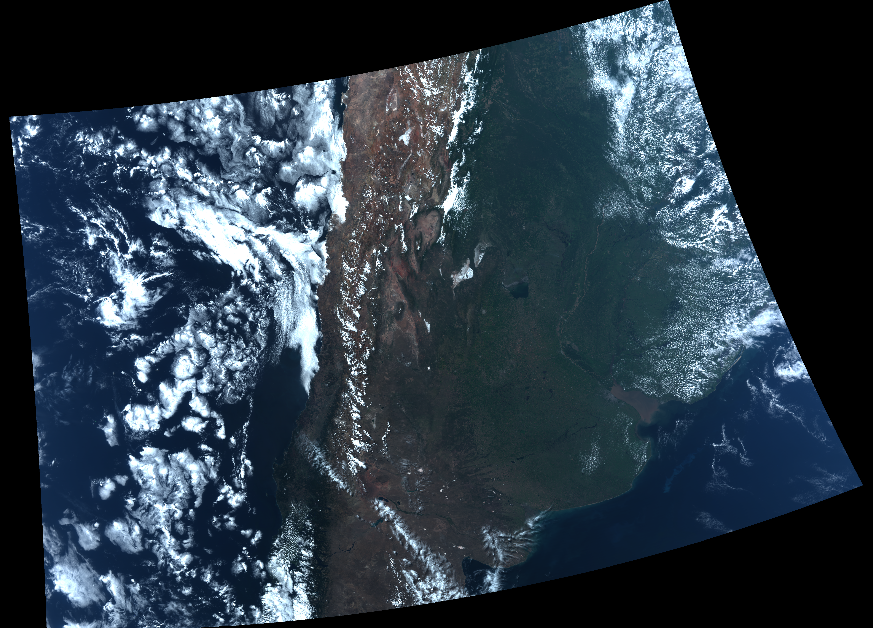
\includegraphics[scale=0.4,keepaspectratio=true,clip=true]{imagenes/recoleccion/img-543.png}
  \caption{Combinación de bandas M5, M4 y M3}
	\label{Fig: bandas543}
\end{figure}



\section{Protocolo Experimental}\label{sec:entrenamiento}

Siguiendo el pipeline desarrollado en la sección (Sec: \ref{sec: pipeline}) ya con los datos de entrenamiento se desarrollo la experimentación de los modelos de detección.

\subsection*{Clasificación - Entrenamiento}\label{sub:entr_class}

Para la clasificación y construcción del modelo se utilizo \ac{svm} (Sec: \ref{sub:clasificadores}), cada conjunto de entrenamiento se realizo utilizando regiones positivas y negativas de cada una de las imágenes obtenidas.

En los algoritmos de aprendizaje automático tenemos parámetros que nos permiten optimizar el modelo que estamos entrenando, estos  parámetros se los llama \textit{hiperparámetros}, una de las técnicas mas usada para la optimización de hiperparámetros es la conocida como \textit{Grid Search}, esta técnica nos ayuda a encontrar una combinación óptima de parámetros del modelo. La técnica \textit{Grid Search} busca por fuerza bruta los parámetros definidos previamente y evalúa cada una de las combinaciones posibles entre los mismos logrando obtener la combinación óptima que maximice alguna de las métricas previamente definida, por ejemplo accuracy. 

En nuestro caso como estamos utilizando \ac{svm} (Sec: \ref{sub:clasificadores}) los hiperparámetros que debemos optimizar son \textit{C} y $\gamma$. El valor de \textit{C} controla el costo del error en la clasificación, \textit{miss classification} en ingles, dado un valor de \textit{C} pequeño hará que el optimizador busque un hiperplano de separación de mayor margen, incluso si ese hiperplano clasifica erróneamente más puntos, con valores grandes de \textit{C}  elegirá un hiperplano de menor margen, el objetivo es encontrar el equilibrio entre "no demasiado estricto" y  "no demasiado relajado". El otro hiperparámetro a  optimizar es el de  $\gamma$ este hiperparámetro es la inversa de la desviación estándar de un kernel \textit{RBF} (función gaussiana), que se utiliza como medida de similitud entre dos puntos.
El rango de hiperparámetros utilizados para entrenar el modelo con \textit{Grid Search} fueron los siguientes: \textit{Tipos de kernel}: lineal y RBF (gaussiano); para rango de valores de \textit{C}: $(10^{3}, 10^{2}, 10^{1}, 10^{0}, 10^{-1},10^{-2}, 10^{-3}, 10^{-4})$
    y para rango de valores de $\gamma$: $(1,0,10^{-1}, 10^{-2},10^{-3},10^{-4}. 10^{-5})$
    
Para evitar el overfitting (Sec:\ref{sub:problema_deteccion}) se utilizo \textit{k-fold cross-validation} (Sec:\ref{sub:validacion-modelo}) que en conjunto con \textit{Grid Search} para cada  iteración realizada por la técnica de \textit{Grid Search} se toma un subconjunto de los datos para realizar su validación; en todos los experimentos que se realizaron se utilizo un valor de $K = 5$.


\subsection*{Evaluación del modelo}\label{sub:evaluacion_class}

Para cuantificar la performance de un modelo de detección debemos evaluarlo usando las métricas desarrolladas en la sección (Sec: \ref{sub:evaluación-modelo}) estas son: \textit{precisión}, medida de cuantas predicciones positivas fueron verdaderas; \textit{recall}, nos indica la cobertura en la que el modelo predijo como positivo; \textit{accuracy}, obtenemos la exactitud del modelo; otra de las métricas desarrolladas para evaluar el modelo es a través de las \textit{curvas ROC}, esta curva nos representa la capacidad que tiene modelo entrenado en discriminar entre clases positivas y negativas.

El dataset utilizado para evaluar los modelos entrenados  consta de 10 imágenes, considerando el conjunto de imágenes con la combinación de banda correspondiente, cada una con un promedio de 1500 bounding boxes por imágenes repartidas en regiones tanto negativas como positivas.


En el siguiente cuadro \ref{tab:entrenam-result} se expone los resultados obtenidos de la validación de los modelos entrenados. En la columna \textit{bandas} describe la combinación de banda usada para el experimento; las columnas  de los hiperparámetros nos muestra los valores óptimos encontrados en el entrenamiento a través de algoritmo \textit{Grid Search} y \textit{k-fold cross-validation} , por ultimo tenemos las columnas relacionadas a las métricas finales obtenida en la validación de cada uno de los experimentos ejecutados.


\begin{table}[H]
\begin{center}
\begin{tabular}{|c|c|c|c|c|c|c|c|}
\hline
 & \multicolumn{3}{c|}{Hiperparámetros seleccionado} & \multicolumn{4}{c|}{Metricas} \\ \hline
Bandas & C & $\gamma$ & kernel & precision & recall & \begin{tabular}[c]{@{}c@{}}average\\ precision \end{tabular} & \begin{tabular}[c]{@{}c@{}}mean overlap \end{tabular} \\ \hline
\multicolumn{1}{|c|}{1-1-1} & 10 & - & linear & 0.83 & 0.91 & 0.54 & 0.1 \\ \hline
\multicolumn{1}{|c|}{1-3-5} & 10 & - & linear & 0.93 & 0.94 & 0.67 & 0.28 \\ \hline
\multicolumn{1}{|c|}{\textbf{1-5-3}} & \textbf{1000} & \textbf{0.01} & \textbf{rbf} & \cellcolor{yellow!50}\textbf{0.95} & \cellcolor{yellow!50}\textbf{0.95} & 0.73 & 0.27\\ \hline
\multicolumn{1}{|c|}{3-1-5} & 100 & 0.01 & rbf & 0.93 & 0.95 & 0.72 & 0.31 \\ \hline
\multicolumn{1}{|c|}{3-3-3} & 1000 & 1 & rbf & 0.92 & 0.92 & 0.28 & 0.1 \\ \hline
\multicolumn{1}{|c|}{3-5-1} & 10 & 0.01 & rbf & 0.90 & 0.91 & 0.66 & 0.25 \\ \hline
\multicolumn{1}{|c|}{5-1-3} & 1 & 1 & rbf & 0.89 & 0.86 & 0.46 & 0.29 \\ \hline
\multicolumn{1}{|c|}{5-3-1} & 1000 & 0.001 & rbf & 0.90 & 0.88 & 0.38 & 0.21 \\ \hline
\multicolumn{1}{|c|}{5-5-5} & 100 & 0.01 & rbf & 0.89 & 0.85 & 0.63 & 0.26 \\ \hline
\multicolumn{1}{|c|}{7-7-7} & 1000 & 0.001 & rbf & 0.92 & 0.92 & 0.75 & 0.30 \\ \hline
\multicolumn{1}{|c|}{9-9-9} & 10 & 1 & rbf & 0.82 & 0.75 & 0.34 & 0.1 \\ \hline
\multicolumn{1}{|c|}{11-7-9} & 1000 & 0.001 & rbf & 0.91 & 0.86 & 0.59 & 0.24 \\ \hline
\multicolumn{1}{|c|}{11-9-7} & 10 & - & linear & 0.91 & 0.89 & 0.74 & 0.26 \\ \hline
\multicolumn{1}{|c|}{7-11-9} & 1 & 1 & rbf & 0.91 & 0.87 & 0.60 & 0.27 \\ \hline
\multicolumn{1}{|c|}{7-9-11} & 10 & - & linear & 0.90 & 0.89 & 0.73 & 0.28 \\ \hline
\multicolumn{1}{|c|}{9-11-7} & 1 & 1 & rbf & 0.89 & 0.86 & 0.66 & 0.23 \\ \hline
\multicolumn{1}{|c|}{9-7-11} & 1 & 1 & rbf & 0.89 & 0.86 & 0.79 & 0.30\\ \hline
\multicolumn{1}{|c|}{11-11-11} & 1 & 1 & rbf & 0.91 & 0.88 & 0.74 & 0.27 \\ \hline
\multicolumn{1}{|c|}{11-3-15} & 10 & 0.1 & rbf & 0.89 & 0.83 & 0.59 & 0.3 \\ \hline
\multicolumn{1}{|c|}{11-15-13} & 1 & 1 & rbf & 0.89 & 0.84 & 0.63 & 0.28 \\ \hline
\multicolumn{1}{|c|}{13-11-15} & 10 & - & linear & 0.89 & 0.87 & 0.61 & 0.26 \\ \hline
\multicolumn{1}{|c|}{13-13-13} & 1 & - & linear & 0.91 & 0.90 & 0.32 & 0.35 \\ \hline
\multicolumn{1}{|c|}{13-15-11} & 1 & - & linear & 0.89 & 0.82 & 0.39 & 0.26 \\ \hline
\multicolumn{1}{|c|}{15-11-13} & 10 & 1 & rbf & 0.89 & 0.86 & 0.51 & 0.25 \\ \hline
\multicolumn{1}{|c|}{15-13-11} & 1000 & 0.001 & rbf & 0.90 & 0.86 & 0.54 & 0.27 \\ \hline
\multicolumn{1}{|c|}{15-15-15} & 10 & 1 & rbf & 0.88 & 0.85 & 0.26 & 0.28 \\ \hline
\multicolumn{1}{|c|}{11-12-13} & 1000 & 1 & rbf & 0.87 & 0.91 & 0.62 & 0.32 \\ \hline
\multicolumn{1}{|c|}{5-4-3} & 1000 & 1 & rbf & 0.88 & 0.87 & 0.57 & 0.27 \\ \hline
\multicolumn{1}{|c|}{\textbf{10-7-5}} & \textbf{1000} &\textbf{ 0.001} & \textbf{rbf} & 0.91 & 0.96 &\cellcolor{blue!25}\textbf{0.93} & \cellcolor{blue!25}\textbf{0.36}\\ \hline
\end{tabular}
\end{center}\caption{Resultados.}\label{tab:entrenam-result}
\end{table}

En base a los resultados obtenidos de cada entrenamiento expuesto en la tabla \ref{tab:entrenam-result} existen diversas combinaciones de bandas en la cual se obtienen mejores métricas de precision, recall, average precision y mean overlap con respecto a otra.  

En las combinaciones de bandas \textbf{1-5-3} se puede ver que se obtuvo métricas en comparación con el resto mayores en precision como en recall, esto nos dice que el modelo entrenado con esta banda predijo con una precisión de  $94\%$  si la región buscada era la región de interés y con un error del $6\%$ el modelo se equivoco al predecir como verdadero una región que no era del área de interés (falso positivo), de la misma forma el recall para esta banda nos indica que en un $6\%$ no se logro detectar regiones de interés. En los falsos positivos detectados se observo en todo los casos que debido a la naturaleza de la imagen el modelo tiende a confundirse con las nubes blancas como se puede observar en la imagen (a) \ref{fig:COMB_BANDAS}.

Se pudo observar que la mayoría de las combinaciones de bandas que presentan \textit{average precision} (AP), medida que calcula  el área bajo la curva entre precisión y recall, mayor a $70\%$ la naturaleza de las imágenes son muy idénticas como se puede observar en la figura (a) \ref{fig:COMB_BANDAS} y (b) \ref{fig:COMB_BANDAS}; para dar un ejemplo de esta medida, cada 10 regiones positivas se detectaron $8$ regiones. Por otro lado se observa que en la mayoría de los casos donde el modelo detecto \textit{falsos positivos} se debió al contraste entre las nubes y el suelo o agua.



Por ultimo analizamos la combinación de bandas \textbf{10-7-5} (c) (Fig:\ref{fig:COMB_BANDAS}) (color verdadero o por su nombre en ingles \textit{True color}), en esta combinación de bandas se obtuvieron los mejores resultados en cuanto a las métricas de AP (average precision) y  \textit{mean overlap}, esta ultima medida se calcula la intersección sobre unión \textit{IoU} de las regiones, el resultado nos dice que tan exacto es el modelo en cuanto a precisión en términos de localización de la región. Con esta combinación de banda el modelo supo generalizar logrando aprender las características del \textit{ground thruth} en la imagen, como se puede ver en la misma posee diferentes tonalidades del suelo así también a simple vista se puede detectar los diferentes contraste que hay entre las nubes, suelo o agua, estas características particulares hacen que permita identificar de manera adecuada las diferentes clases que estamos buscando.

\begin{figure}[htbp]
\centering
\subfigure[]{\includegraphics[scale=0.2]{imagenes/evaluacion/1-5-3.png}}
\subfigure[]{\includegraphics[scale=0.2]{imagenes/evaluacion/9-7-11.png}}
\subfigure[]{\includegraphics[scale=0.2]{imagenes/evaluacion/10-7-5.png}}
\caption{Combinaciones de bandas: (a) bandas 1-5-3, (b) bandas 9-7-11, (c) bandas 10-7-5} \label{fig:COMB_BANDAS}
\end{figure}

Para realizar un análisis mas detallado de la performance de los modelos entrenados se seleccionaron aquellos que tienen mejores métricas con respecto al resto analizando las \textit{curvas ROC} esta permite ver la capacidad del modelo entrenado en discriminar las diferentes clases. En el grafico \ref{fig:Average_precision} se puede visualizar para todas las curvas ROC a medida que aumenta el valor de \textit{recall} va disminuyendo la \textit{precision}. El objetivo es identificar aquel valor que aumente el recall sin perder la precision.
\newpage

Para las bandas 1-5-3 (Fig: \ref{fig:Average_precision} (a)) el valor optimo se da cuando la precision esta en $0.9$ y $0.2$ en recall, esto nos indica que el modelo entrenado tiene un porcentaje alto de precision a la hora de clasificar una nueva imagen pero un recall bajo ya que no captura todas las regiones dentro de la imagen de igual manera para las bandas 9-7-11 (Fig:\ref{fig:Average_precision} (b)) el valor observado optimo esta dado entre la precision $0.9$ y recall $0.4$, siendo este ultimo valor mas optimo en relación a las bandas 1-5-3. Por ultimo las bandas 10-7-5 (Fig: \ref{fig:Average_precision} (c)) se puede observar que el modelo generalizo de manera optima logrando capturar las características de las imágenes es por esto que se obtuvo una precision de $0.9$ y recall  de $0.8$, siendo este el modelo entrenado mas óptimo. 

\begin{figure}[htbp]
\centering
\subfigure[]{\includegraphics[scale=0.40]{imagenes/evaluacion/ROC153.png}}
\subfigure[]{\includegraphics[scale=0.40]{imagenes/evaluacion/AP9711.png}}
\subfigure[]{\includegraphics[scale=0.40]{imagenes/evaluacion/ROC1075.png}}
\caption{Curvas ROC, average presicion para diferentes set de bandas, (a) bandas 1-5-3, (b) bandas 9-7-11, (c) bandas 10-7-5} \label{fig:Average_precision}
\end{figure}
 
Como se observo en los diferentes experimentos realizados, las imágenes construidas con diferentes bandas nos brindan diversas fuente de información que nos permiten construir y mejorar los modelos de \ac{ml}. El principal inconveniente detectado en todos los modelos entrenados con las diferentes combinaciones de bandas fueron las nubes en las imágenes, la mayoría de los \textit{falsos positivos} detectados se debió a la presencia de las misma; por otro lado se observa en la tabla \ref{tab:entrenam-result} que las combinaciones de bandas que mayor métricas dieron fueron aquellas que de alguna manera se podía distinguir y resaltar el suelo, agua y nubes, esto se puede ver reflejado en las bandas  \textbf{1-1-1} (fig: \ref{Fig:imagen_banda_111}) en donde no se puede distinguir las regiones de interés dentro de la misma. 
 
 \begin{figure}[H]\centering
  \includegraphics[scale=0.3,keepaspectratio=true,clip=true]{imagenes/evaluacion/1-1-1.png}
  \caption{Combinación de bandas 1-1-1} \label{Fig:imagen_banda_111}
\end{figure}
 
Para finalizar la evaluación experimental se predijo a modo de ejemplo una imagen nunca vista por los modelos entrenados, en este caso utilizamos el modelo entrenado con las bandas \textbf{9-7-11} para realizar la predicción, en la figura siguiente  \ref{Fig: TP} se pude visualizar el resultado de la misma.

\begin{figure}[H]\centering
  \includegraphics[scale=0.05,keepaspectratio=true,clip=true]{imagenes/evaluacion/prediction-9711.png}
  \caption{Predicción modelo - bandas 9-7-11} \label{Fig: TP}
\end{figure}

%http://rammb.cira.colostate.edu/projects/npp/VIIRS_bands_and_bandwidths.pdf













